\title{CS 472 HW 7}
\author{
        Aaron Havens\\
}
\date{\today}

\documentclass[12pt]{article}
\usepackage{amssymb} %maths
\usepackage{amsmath} %maths
\usepackage{graphicx}
\usepackage{array}
\usepackage{subfig}
\graphicspath{{figs/}}
\begin{document}
\maketitle\

\paragraph{14.1)}
a.)\\
\begin{figure}[h]
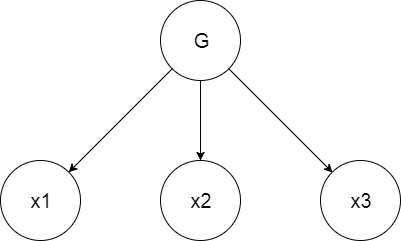
\includegraphics[scale=.5]{graph}
\end{figure}

\begin{figure}
\centering
\subfloat[The CPC for G]{\begin{tabular}{|c|c|} 
\hline
G&P(G)\\ [0.5ex] 
\hline
a & 1/3\\
\hline
b & 1/3\\
\hline
c & 1/3\\[1ex] 
 \hline
\end{tabular}}
\qquad
\subfloat[The CPC for $x_i$ given G]{\begin{tabular}{|c|c|c|} 
\hline
G&$X_i$&P(G)\\ [0.5ex] 
\hline
a & heads&0.2\\
\hline
b & head&0.6\\
\hline
c & heads&0.8\\[1ex] 
 \hline
\end{tabular}}
\end{figure}
b.) First apply Bayes Rule to reverse the dependency.
\begin{align}
P(G|\text{2 heads, 1 tail}) = P(\text{2 heads, 1 tails}|G)P(G)/P(\text{2 heads, 1 tails})\\
P(\text{2 heads, 1 tails}|G)
\end{align}
$x_1, x_2$ and $x_3$ are conditionally independent of given G (they are d separated by G). The highest conditionally probability in question can then calculated, where there are 3 choose 2 combinations of the event for a.
\begin{align}
P(x_1 = tails | G = a)P(x_2 = heads|G = a)P(x_3 = heads|G = a) = 0.032\\
P(\text{2 heads, 1 tails}| G = a) = 3 * 0.032 = 0.096\\
\end{align}
It follows that.
\begin{align}
P(\text{2 heads, 1 tails} | G = b) = 0.432\\
P(\text{2 heads, 1 tails} | G = c) = 0.384\\
\end{align}
The condition $G=b$ provides the highest conditionally probability.
\paragraph{14.6)}
a). The network c represent represents the expression. The independence of genes is asserted.\\
b). a and b both consistent with the claim. However, b may have some unnecessary dependencies based on the description.\\
c.) a is the best representation for reasons stated above.\\
d.) 
\begin{table}[h]
\begin{center}
\caption{CPC for handedness} \label{tab:title} 
\begin{tabular}{|c c|c c|} 
\hline
$G_{mother}$&$G_{father}$&P($G_{child} = l$| --)&P($G_{child} = r$| --)\\ [0.5ex] 
\hline
l & l&1-m&m\\
\hline
l & r&0.5&0.5\\
\hline
r & l&0.5&0.5\\ 
\hline
r&r&m&1-m\\[1ex]
\hline
\end{tabular}
\end{center}
\end{table}
\\
e.) 
\begin{align}
P(G_{child}=l) = \sum_{g_m,g_f} P(G_{child} = l|g_m,g_f)P(g_m,g_f)\\
= \sum_{g_m,g_f} P(G_{child} = l | g_m, g_f)P(g_m)P(g_f)\\
=(1-m)q^2 + 0.5q(1-q)+0.5(1-q)q+m(1-q)^2\\
=q+m-2mq
\end{align}
f.) left-handedness is humans is fairly uncommon ($\approx 10\%$ according to Google). For equilibrium, $P(G_{child} = l) = P(G_{mother}=l) = P(G_{father}=l)$. This implies that $q+m-2mq=q, \quad q = 0.5$. This seems too high for current global statistics.
\paragraph{14.14)}
a.) 
ii, and iii are asserted by the network.
b.)$P(b,i,\neg m,g,j)=P(b)P(\neg m)P(i|b,\neg m)P(g|b,i,\neg m)P(j|g) = 0.9 * 0.9 * 0.5 * 0.8 * 0.9 = 0.2916$\\
c.) B, I and M are given as evidence with values of \textit{true}. This gives G a prior of $0.9$. The probability of going to jail is:
\begin{align}
P(J|b,i,m) = \alpha \sum_g P(J,g) \\
= \alpha (P(J,g)+P(J,\neg g))\\
= \alpha (\langle P(j,g), P(\neg j,g) \rangle + \langle P(j,\neg g),P(\neg j, \neg g) \rangle ) \\
= \langle 0.81, 0.19 \rangle\\
=\alpha (\langle 0.81, 0.09 \rangle + \langle 0,0,1 \rangle ) = \langle 0.81, 0.19 \rangle
\end{align}
The probability of jail is 0.81.\\
Markov Blanket for variable M in the network includes M's parents, children and its childrens' other parents: ${I,G,B}$
\end{document}